% The document will be printed one side in A4 paper.
%\documentclass[12pt,a4paper,oneside]{report}
%\documentclass[12pt,a4paper,twoside]{report}
\documentclass[12pt,a4paper,twoside]{article}


\usepackage[round]{natbib}

\usepackage[pdftex]{color,graphicx}
\usepackage{setspace}
\usepackage{a4wide}

\usepackage[a4paper]{geometry}
\usepackage[cm]{fullpage}


%subfigures deprecated
%\usepackage{subfigure}
%use subcaption instead
\usepackage{caption}
\usepackage{subcaption}
%side caption: SCfigure
%\usepackage{sidecap}
% Use PDF output.
% The output should be wide.
\usepackage{url}
%for definition list
\usepackage{enumitem}
%for celsius
%\usepackage{gensymb}
%for listing code
\usepackage{listings}
%for table cell with diagonal division
\usepackage{slashbox}
\usepackage{tabularx}
\usepackage{amsmath}

%\usepackage[graphics,tightpage,active]{preview}
%\PreviewEnvironment{tikzpicture}
%\PreviewEnvironment{equation}
%\PreviewEnvironment{equation*}
%\newlength{\imagewidth}
%\newlength{\imagescale}
%\pagestyle{empty}
%\thispagestyle{empty}
%\usepackage{standalone}

\usepackage[french, greek, english]{babel}
%input encoding
%\usepackage[iso-8859-7]{inputenc}
%\usepackage[latin1]{inputenc}
%output encoding
\usepackage[T1]{fontenc}
\selectlanguage{english}

% Pour la dedicace
\usepackage{frcursive}

\usepackage[table]{xcolor}
\usepackage{booktabs}
\usepackage{tabu}

\usepackage[section,subsection,subsubsection]{extraplaceins}
\usepackage{url} %tablerules
\usepackage{xr}
\externaldocument{supplementary}

\usepackage[labelfont=bf,labelsep=period,justification=raggedright]{caption}

\usepackage{xr}
\externaldocument{paper}

\setcounter{secnumdepth}{0}


%\doublespacing

\title{ Supplementary }
%\texttt{nikolas.pontikos@cimr.cam.ac.uk}\\
\date{}

%\renewcommand\listfigurename{Supplementary Figures}
%\renewcommand\listtablename{Supplementary Tables}


\begin{document}

\maketitle
\noindent

\renewcommand\figurename{Supplementary Figure}
\renewcommand\tablename{Supplementary Table} 




%\section{SNP Copy Number Calling}



\section{Figures}

\begin{figure}[h]
%\begin{center}
    \centering
    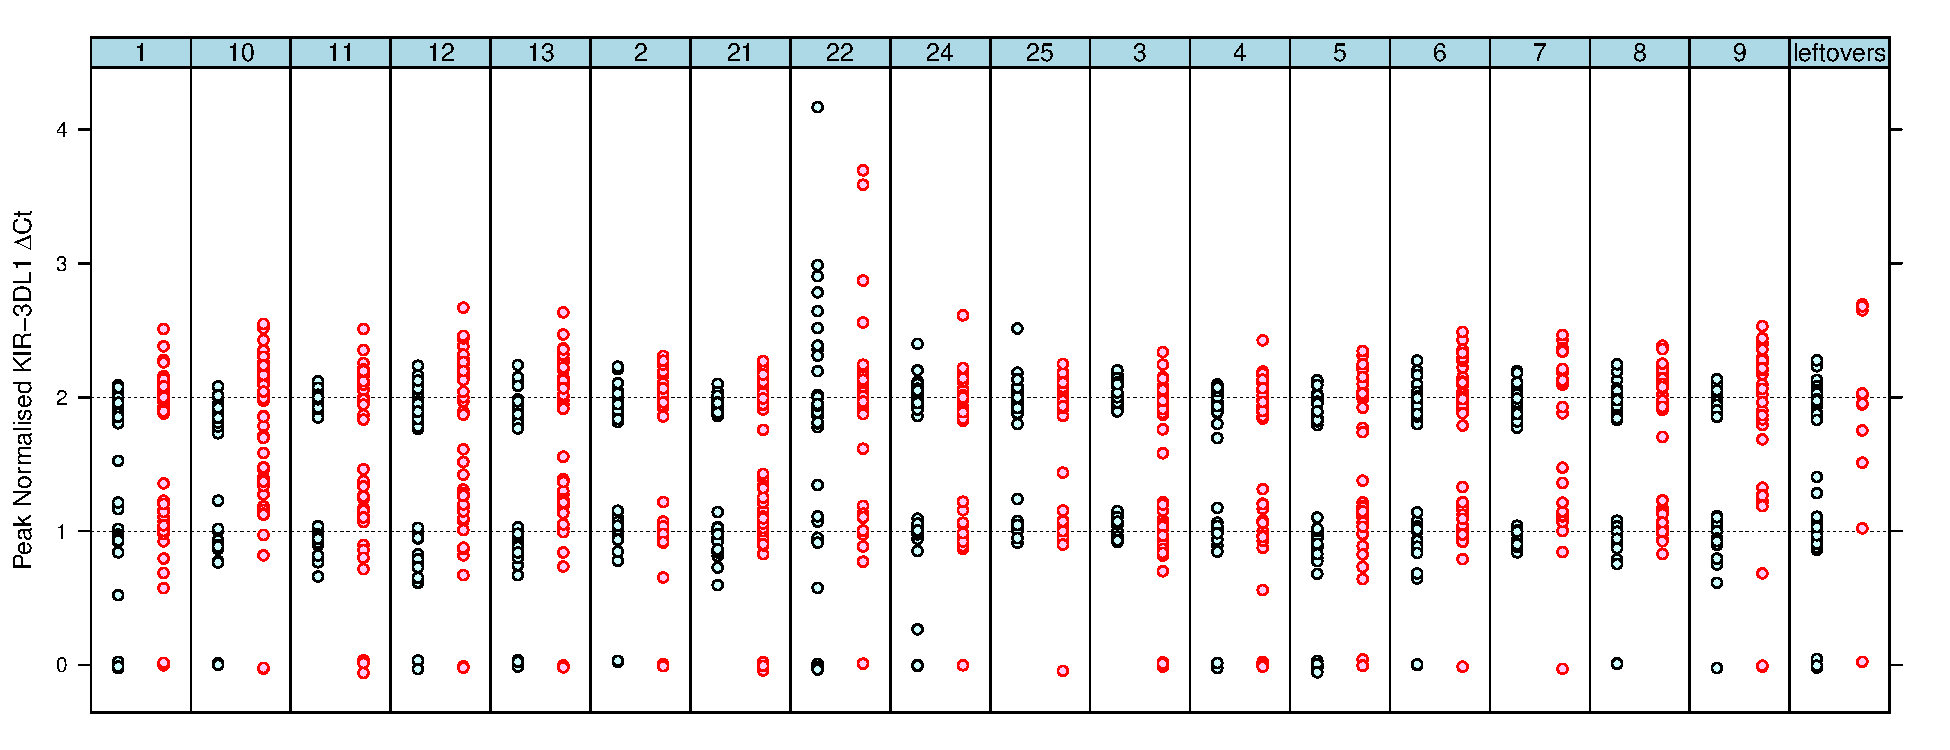
\includegraphics[scale=.5] {figures/normalised-median.pdf}
    \caption{
        Post-QC normalised \emph{KIR3DL1} $\Delta$Ct values for cases (red) and controls (blue) per plate.
        Plate 22 stands out as the noisiest for \emph{KIR3DL1} which suggests it should be excluded from the analysis.
    }
    \label{figure:normalised-median}
\end{figure}


\begin{figure}[h]
%\begin{center}
    \centering
    \begin{subfigure}[b]{.4\textwidth}
        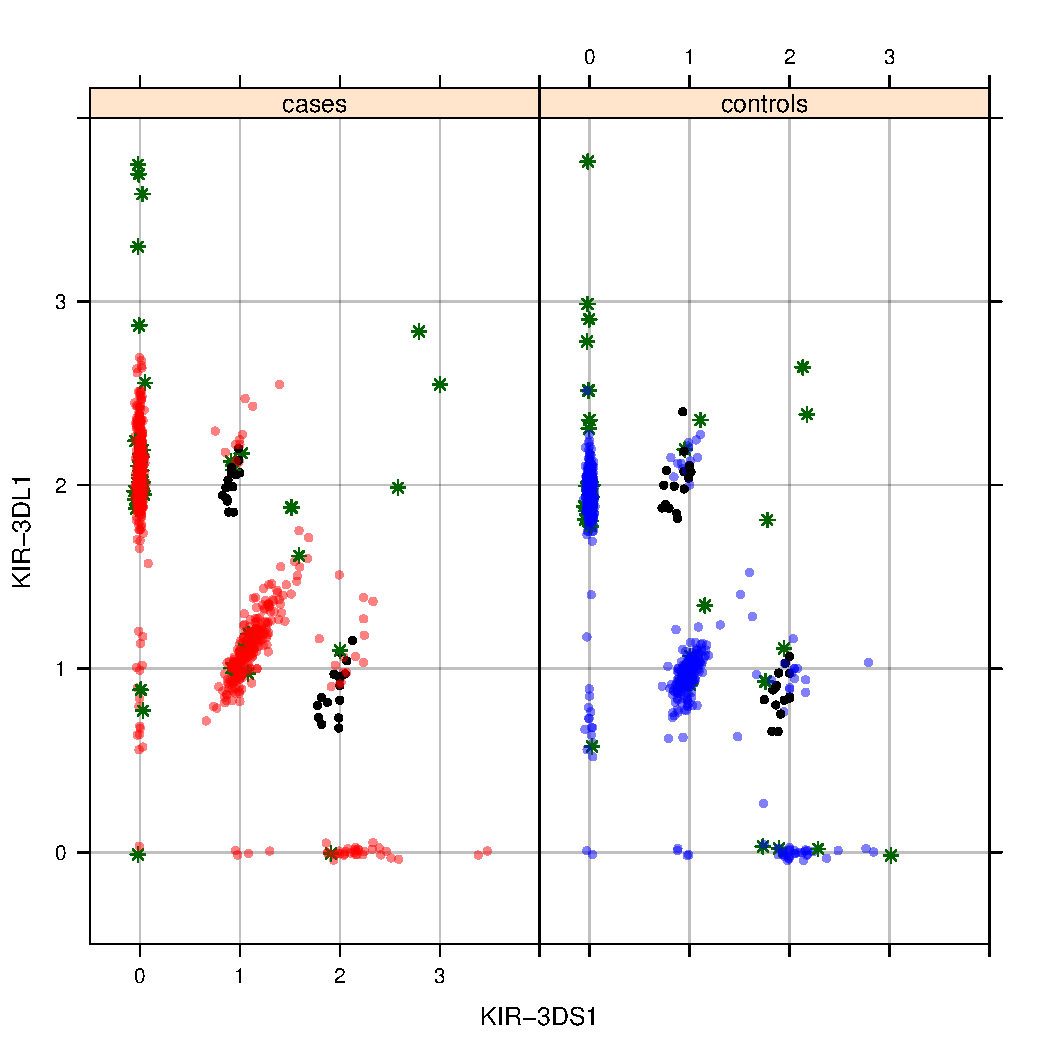
\includegraphics[scale=.4] {figures/qc1.pdf}
        \caption{Pre QC: 816 cases (red) and 813 controls (blue).}
    \end{subfigure}
    ~
    \begin{subfigure}[b]{.4\textwidth}
        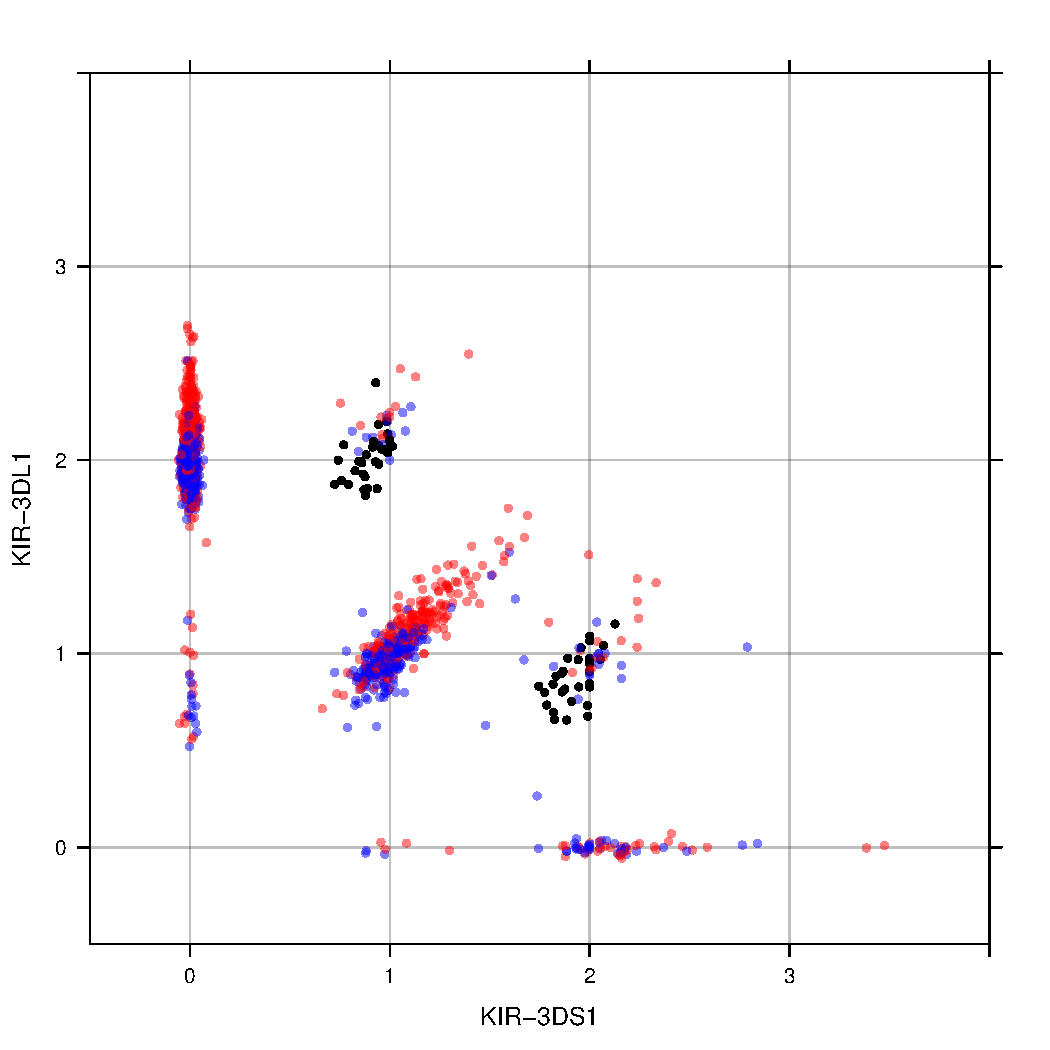
\includegraphics[scale=.4] {figures/qc4.pdf}
        \caption{Post QC: 747 cases (red) and 727 controls (blue).}
        \label{}
    \end{subfigure}
    \caption{
        \label{figure:QC}
        (a) Cases are in red, controls are in blue and the samples with known \emph{KIR3DL1/S1} copy number are in black.
        Samples from plate 22 are represented by the green asterisks.
        There is a larger spread in cases than in controls for 3DL1.
        QC involved dropping plate 22 which is very noisy and samples for which we do not have four replicates.
        (b) After QC we are left with a total of 1,474 unique samples (747 cases and 727 controls).
    }
\end{figure}



\begin{figure}[h]
%\begin{center}
    \centering
    \begin{subfigure}[b]{.4\textwidth}
        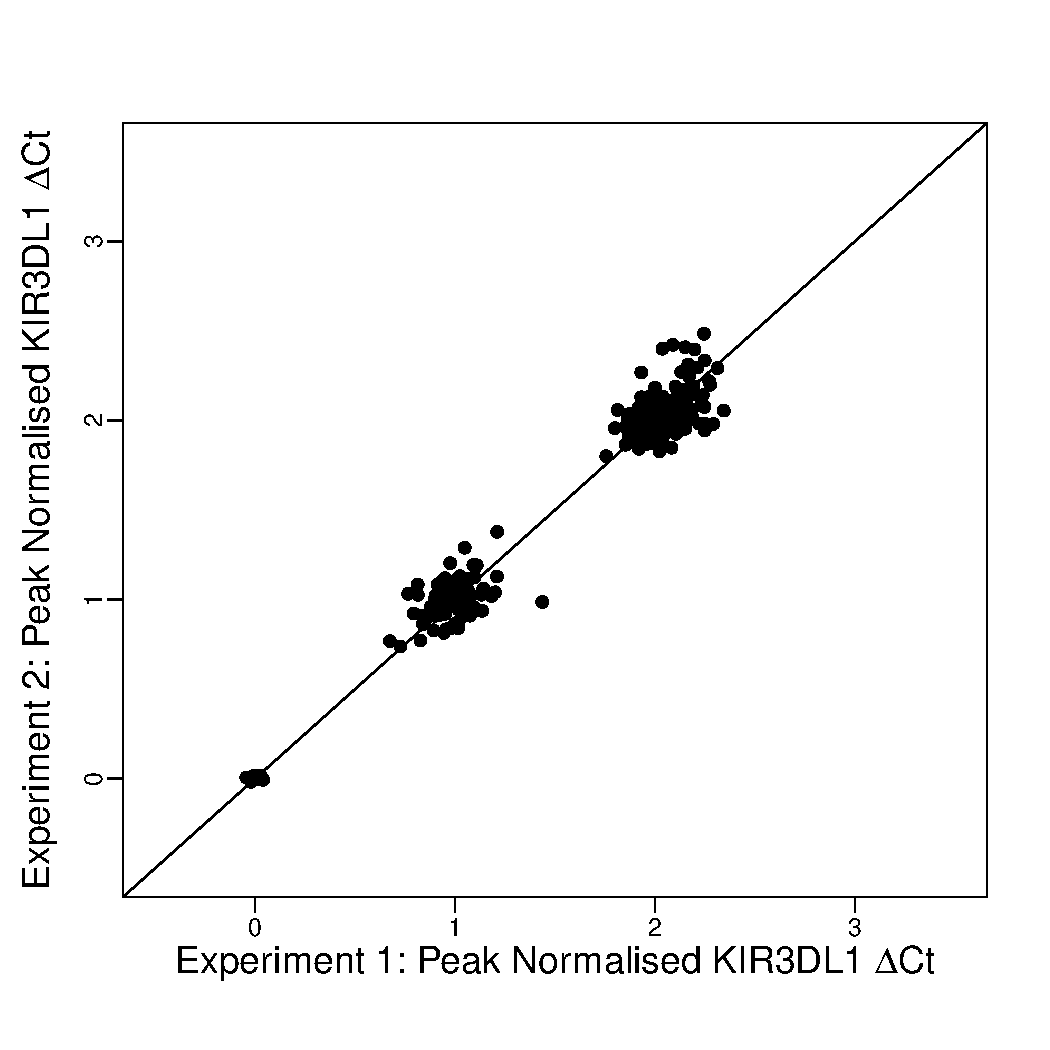
\includegraphics[scale=.4] {figures/DL1-repeatability.pdf}
        \caption{Repeatability of KIR3DL1 $\Delta$Ct post normalisation and QC ($r^{2}=0.961$).}
    \end{subfigure}
    ~
    \begin{subfigure}[b]{.4\textwidth}
        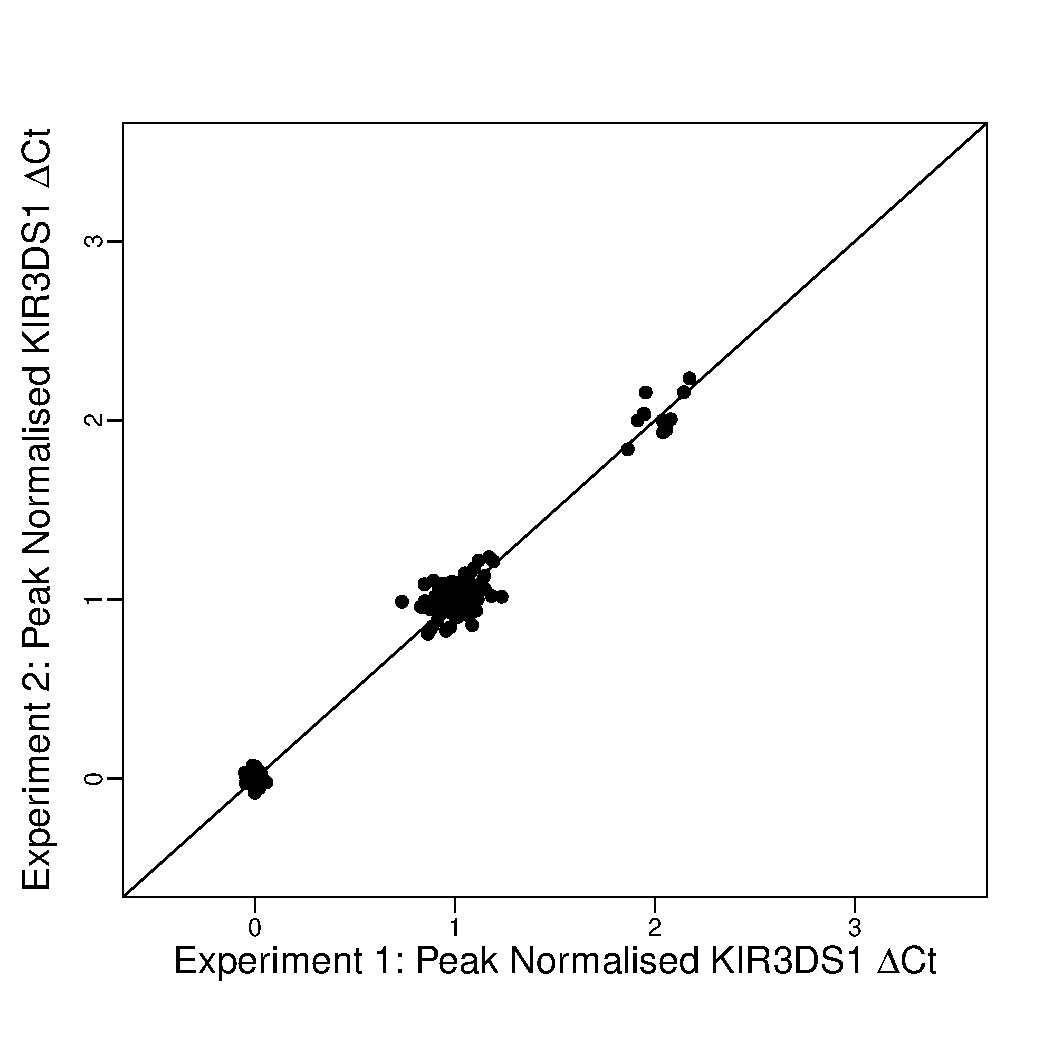
\includegraphics[scale=.4] {figures/DS1-repeatability.pdf}
        \caption{Repeatability of KIR3DS1 $\Delta$Ct post normalisation and QC ($r^{2}=0.99)$.}
        \label{}
    \end{subfigure}
    \caption{
        \label{figure:repeatability}
        In order to assess the reliability of the qPCR assay 310 samples were re-analysed.
        We found very high reproducibility of the $\Delta$Ct values ($r^{2} > 0.96)$ confirming the reliability of our qPCR assay.
        %Samples on four plates were repeated to assess 
        %The points are coloured by genotype group as defined in Figure~\ref{figure:fuzzy-genotyping}.
        %302 samples
    }
\end{figure} 




\begin{figure}[h]
%\begin{center}
    \centering
    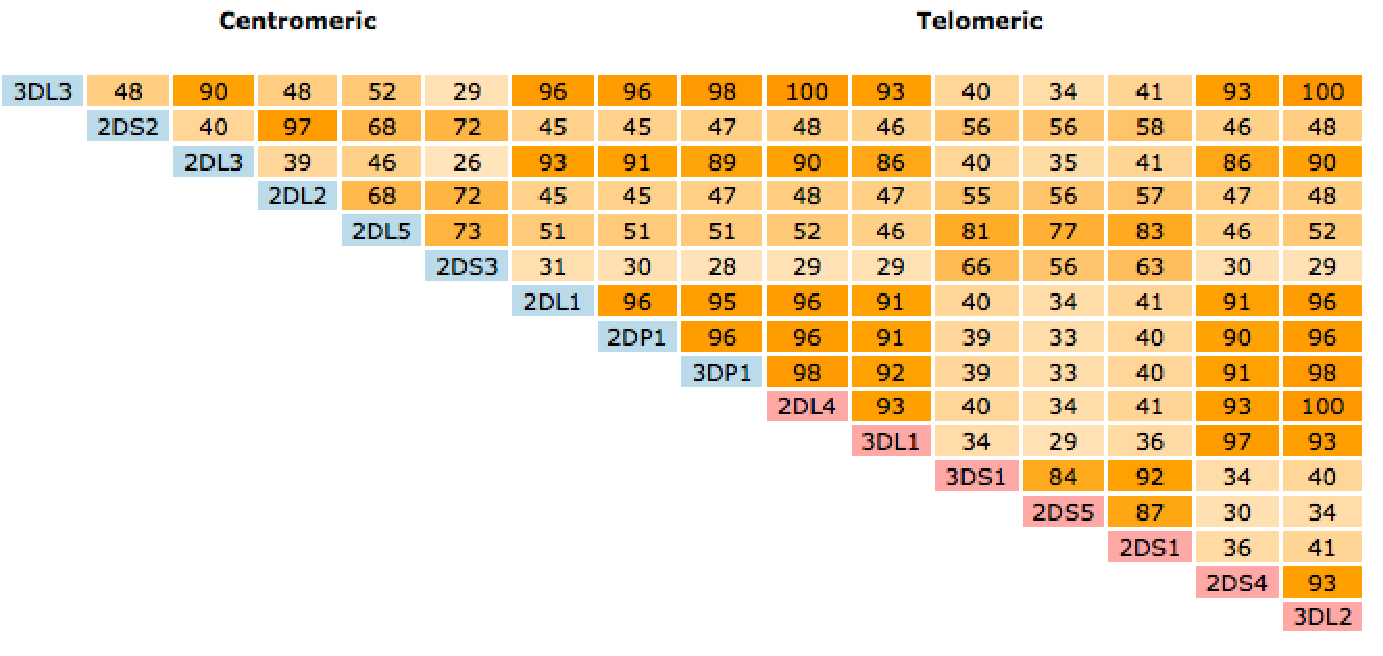
\includegraphics[scale=.75] {figures/LD.pdf}
    \caption{
        Linkage values 0-100\% between KIR genes organised by telomeric (blue) and centromeric (red) content.
        Gene association values are estimated using the genotype list which is available on the Allele Frequencies Net website \citep{GonzalezGalarza:2011gm}.
        %at \url{http://www.allelefrequencies.net/kir6010a.asp}
    }
    \label{figure:LD}
\end{figure}




\section{Tables}



\begin{table}[h]
\begin{center}
\footnotesize
\begin{tabular}{lll}
    \toprule
%\hline
    Gene & Oligos & Sequence (5'-3') \\
\midrule
    & Forward Primer & \texttt{CATCGGTTCCATGATGCG} \\
    3DS1 & Reverse Primer & \texttt{GGGAGCTGACAACTGATAGG} \\
    & Probe & \texttt{AACAGAACCGTAGCATCTGTAGGTCCCT} \\
\midrule
    & Forward Primer & \texttt{CACAGTTGGATCACTGCGT} \\
    3DL1 & Reverse Primer & \texttt{CCGTGTACAAGATGGTATCTGTA} \\
    & Probe & \texttt{CCCTTCTCAGAGGCCCAAGACAC} \\
\midrule
    & Forward Primer & \texttt{CCAGATGCCTACCATGGTG} \\
    STAT6 & Reverse Primer & \texttt{CCATCTGCACAGACCACTCC} \\
          & Probe & \texttt{CTGATTCCTCCATGAGCATGCAGCTT} \\
\end{tabular}
\end{center}
    \caption{
        The qPCR primers used. These were originally developed by \citet{Jiang:2012cf}.
    }
    \label{table:qPCR-primers}
\end{table}


\begin{table} [h]
\begin{center}
\footnotesize
\begin{tabularx} {\linewidth} {l l l X X}
\toprule
Epitope & & Residues (77-83) & HLA-B & HLA-A \\
\midrule
HLA-Bw4 & 80I & {\tt{NLR{\bf{I}}ALR}} & B*1516 B*1517 B*1524 B*2702 B*3801 B*4901 B*5101 B*5108 B*5201 B*5301 B*5302 B*5701 B*5702 B*5801 & A*2301 A*2402 A*2403 A*2407 A*2501 A*3201 \\
\midrule
HLA-Bw4 & 80T & {\tt{DLR{\bf{T}}LLR}} & B*1302 B*2701 B*2704 B*2705 B*3701 B*3802 B*4402 B*4403 B*4404 B*4405 B*4414 B*4417 B*4429 B*4435 B*4701 & \\
\midrule
HLA-Bw6 &  & {\tt{SLR{\bf{N}}LRG}} & B*702 B*703 B*705 B*706 B*708 B*710 B*716 B*726 B*801 B*1401 B*1402 B*1501 B*1503 B*1504 B*1505 B*1507 B*1508 B*1509 B*1510 B*1514 B*1515 B*1518 B*1539 B*1801 B*3501 B*3502 B*3503 B*3508 B*3901 B*3906 B*3928 B*4001 B*4002 B*4006 B*4011 B*4023 B*4101 B*4102 B*4202 B*4501 B*4601 B*4801 B*5001 B*5002 B*5501 B*5601 & \\
\end{tabularx}
\end{center}
    \caption{
        The \citet{Martin:2002el} HLA-Bw4/6 epitope defines the classification of HLA-B and HLA-A alleles based on the amino acid at position 80.
        HLA-Bw4 groups both HLA-Bw4-80I and HLA-Bw4-80T epitopes.
        %\citet{Sidney:2008bn}
        %http://www.dorak.info/hla/bw4bw6.html
    }
    \label{table:HLA-epitope}
\end{table}


\begin{table} [h]
\begin{center}
\footnotesize
\begin{tabular}{rccc}
  \hline
  HLA Epitope & Cases & Controls & Total \\
  \hline
    N/A & 3822 (11) & 2681 (70) & 6503 (81) \\
    \hline
    HLA-Bw6 & 1175 (308) & 753 (199) & 1928 (507) \\
    HLA-Bw4-80T  & 651 (162)  & 754 (174) & 1405 (336) \\
    HLA-Bw4-80I & 1096 (266) & 1174 (284) & 2270 (550) \\
    \hline
    %Total & 6744 (747) & 5362 (727) & 12106 (1474) \\
    HLA total & 2922 (736) & 2681 (657) & 5603 (1393) \\
\end{tabular}
\end{center}
    \caption{
        HLA epitope classification of subjects in study.
        In parentheses, number of subjects analysed with qPCR post QC.
        No HLA typing was done for the N/A category.
        The HLA epitopes are defined in Table~\ref{table:HLA-epitope}.
        An individual is assigned to an HLA epitope group if he is a carrier of at least one allele of that group.
        So that each individual only belongs to a single HLA epitope group,
        the assignment priority is first HLA-Bw4-80I, then HLA-Bw4-80T and finally HLA-Bw6 allele if no HLA-Bw4 alleles 
        were found.
    }
    \label{table:HLA-typing}
\end{table}




\begin{table}[h]
\begin{center}
\footnotesize
\begin{tabular}{rlrrlllrl}
  \hline
 & Name & Position & Score & SNP & Ill Strand & Cust Strand & NormID & QC \\ 
  \hline
1 & rs597598 & 60007252 & 0.89 & [A/G] & TOP & TOP &   1 & ok \\ 
  2 & rs598452 & 60007428 & 0.86 & [A/G] & TOP & BOT &   1 & ok \\ 
  3 & t1d-19-60007809-C-G & 60007809 & 0.79 & [G/C] & BOT & BOT & 100 & ok \\ 
  4 & rs55761930 & 60008141 & 0.66 & [T/C] & BOT & TOP &   1 & ok \\ 
  5 & rs10500318 & 60012591 & 0.72 & [A/G] & TOP & TOP &   1 & ok \\ 
  6 & rs592645 & 60012739 & 0.68 & [A/T] & TOP & BOT & 100 & ok \\ 
  7 & rs604077 & 60013208 & 0.89 & [A/G] & TOP & BOT &   1 & ok \\ 
  8 & rs604999 & 60013409 & 0.89 & [A/G] & TOP & TOP &   1 & ok \\ 
  9 & t1d-19-60014013-A-C & 60014013 & 0.82 & [T/G] & BOT & TOP &   1 & lowcallrate \\ 
  10 & rs3865507 & 60014188 & 0.80 & [T/G] & BOT & TOP &   0 & ok \\ 
  11 & rs3865510 & 60016051 & 0.87 & [A/C] & TOP & TOP &   1 & ok \\ 
  12 & rs648689 & 60016286 & 0.86 & [A/G] & TOP & BOT &   1 & ok \\ 
  13 & rs649216 & 60016447 & 0.90 & [T/C] & BOT & BOT &   1 & ok \\ 
  14 & rs581623 & 60018551 & 0.86 & [A/G] & TOP & BOT &   0 & ok \\ 
  15 & rs4806568 & 60022568 & 0.41 & [A/G] & TOP & TOP &   1 & lowcallrate \\ 
  16 & rs674268 & 60024002 & 0.64 & [T/C] & BOT & TOP &   1 & lowcallrate \\ 
  17 & rs12461010 & 60024413 & 0.79 & [A/G] & TOP & BOT &   0 & ok \\ 
  18 & rs2295805 & 60028513 & 0.83 & [T/C] & BOT & TOP &   1 & lowcallrate \\ 
  19 & rs12976350 & 60030391 & 0.61 & [T/C] & BOT & BOT &   1 & lowcallrate \\ 
  20 & t1d-19-60034052-C-T & 60034052 & 0.63 & [A/G] & TOP & BOT &   1 & hwe \\ 
  21 & rs4806585 & 60038236 & 0.58 & [T/G] & BOT & TOP &   0 & hwe \\ 
  22 & rs62122181 & 60039178 & 0.22 & [T/C] & BOT & TOP &   1 & lowcallrate \\ 
  23 & rs10422740 & 60052298 & 0.81 & [T/C] & BOT & BOT &   0 & monomorph \\ 
  24 & rs640345 & 60054671 & 0.67 & [A/G] & TOP & BOT &   0 & ok \\ 
  25 & t1d-19-60054973-T-C & 60054973 & 0.69 & [A/G] & TOP & BOT &   1 & ok \\ 
  26 & t1d-19-60056605-A-T & 60056605 & 0.70 & [A/T] & TOP & BOT & 200 & ok \\ 
  27 & t1d-19-60056721-C-T & 60056721 & 0.62 & [A/G] & TOP & BOT &   1 & ok \\ 
  28 & rs10407958 & 60063974 & 0.89 & [T/A] & BOT & BOT & 201 & ok \\ 
  29 & rs1654644 & 60065174 & 0.82 & [T/G] & BOT & BOT &   1 & ok \\ 
  30 & rs3826878 & 60069023 & 0.91 & [A/G] & TOP & TOP &   0 & ok \\ 
\end{tabular}
\end{center}
    \caption{
        The ImmunoChip SNPs which fall in the \emph{KIR3DL1} region according to build36/hg18.
        \emph{KIR3DS1} is missing from build36/h18.
    }
    \label{table:ImmunoChip-SNPs}
\end{table}




%\begin{table}[h]
%\begin{center}
%\footnotesize
%\begin{tabular}{c|cccccccc} 
%\backslashbox{SNP}{qPCR} &0-1&0-2&1-0&1-1&1-2&2-0&2-1&3-0\\
%%\cmidrule(lr){2-9}
%\hline
%0-1&21&2&0&2&0&0&0&0\\
%0-2&0&885&0&5&1&0&0&0\\
%1-0&0&0&3&2&0&2&0&0\\
%1-1&0&2&0&434&0&0&0&0\\
%1-2&0&1&0&2&22&0&2&0\\
%2-0&0&0&0&0&0&52&1&1\\
%2-1&0&1&0&3&1&0&26&0\\
%3-0&0&0&0&0&0&4&0&1\\
%\end{tabular}
%\end{center}
%\caption{
%For each of the ten datasets imputed from qPCR, we applied a k nearest neighbour classifier (k=3) to make the copy number predictions and used
%leave one out cross validation to estimate the misclassification rate.
%The numbers shown are the average of each cell over the ten imputed datasets.
%}
%\label{table:training-errors}
%\end{table}


\begin{table}[ht]
\centering
\begin{tabular}{rr}
  \hline
k &  LOO Error \% \\ 
  \hline
1 & 2.68 \\ 
2 & 2.89 \\ 
\bf{3} & \bf{2.10} \\ 
4 & 2.18 \\ 
5 & 2.29 \\ 
6 & 2.36 \\ 
7 & 2.39 \\ 
8 & 2.44 \\ 
9 & 2.56 \\ 
10 & 2.71 \\ 
11 & 2.89 \\ 
12 & 3.11 \\ 
13 & 3.47 \\ 
14 & 3.62 \\ 
15 & 3.64 \\ 
16 & 3.78 \\ 
17 & 3.85 \\ 
18 & 3.81 \\ 
19 & 3.96 \\ 
20 & 3.89 \\ 
   \hline
\end{tabular}
\caption{
    \label{table:knn-loo}
    Average  leave-one-out (LOO) error rate obtained from running k nearest neighbour for k from 1 to 20 over 10 multiply imputed qPCR datasets.
    The smallest average error rate is $2.10\%$ obtained for k=3.
}
\end{table}


\begin{table}[ht]
\centering
\begin{tabular}{c|cccccccc} 
\backslashbox{SNP}{qPCR} &0-1&0-2&1-0&1-1&1-2&2-0&2-1&3-0\\
  \hline
  0-1 & 23.00 & 0.40 & 0.00 & 0.00 & 0.00 & 0.00 & 0.00 & 0.00 \\ 
  0-2 & 1.00 & 886.30 & 0.00 & 2.00 & 1.00 & 0.00 & 1.00 & 0.00 \\ 
  1-0 & 0.00 & 0.00 & 5.00 & 0.00 & 0.00 & 0.00 & 0.00 & 0.00 \\ 
  1-1 & 0.00 & 2.30 & 2.00 & 434.00 & 2.30 & 0.00 & 2.60 & 0.00 \\ 
  1-2 & 0.00 & 1.00 & 0.00 & 0.00 & 21.30 & 0.00 & 0.10 & 0.00 \\ 
  2-0 & 0.00 & 0.00 & 0.00 & 0.00 & 0.00 & 51.50 & 0.00 & 2.30 \\ 
  2-1 & 0.00 & 0.00 & 0.00 & 0.00 & 2.40 & 1.00 & 27.30 & 0.00 \\ 
  3-0 & 0.00 & 0.00 & 0.00 & 0.00 & 0.00 & 0.80 & 0.00 & 3.40 \\ 
  \hline
\end{tabular}
\caption{
    \label{table:knn-misclassification}
    Using the posterior probabilities obtained from the qPCR genotype calls,
    10 datasets were multiply imputed and each was used for training 
    a k nearest neighbour classifier (k=3) to predict genotype from SNP data.
    This table represents the average over the 10 misclassification tables.
    Each cell along the diagonal shows the average number of matching predictions and the
    cells off the diagonal show the contains the average number of mismatches.
    %The cells in this table sum to 1,474 which is total number of samples used for training.
    The average misclassification rate is $1.5\%$.
    }
\end{table}

\begin{table}[h] \footnotesize
%\begin{center}
    \centering
    \begin{tabularx}{\textwidth}{crrr|rrr}
       & \multicolumn{3}{c}{qPCR} & \multicolumn{3}{c}{SNP} \\
      \toprule
      { KIR3DS1-KIR3DL1} & \multicolumn{3}{c}{count (percentage)} & \multicolumn{3}{c}{count (percentage)} \\
          Copy Number & cases & controls & total & cases & controls & total \\ 
      \hline
      0-2 & 444 (59.44) & 446 (61.35) & 890 (60.38) & 4091 (60.66) & 3220 (60.05) & 7311 (60.39) \\ 
      1-1 & 229 (30.66) & 207 (28.47) & 436 (29.58) & 2056 (30.49) & 1628 (30.36) & 3684 (30.43) \\ 
      2-0 & 26 (3.48) & 28 (3.85) & 54 (3.66) & 231 (3.43) & 223 (4.16) & 454 (3.75) \\ 
      2-1 & 15 (2.01) & 16 (2.2) & 31 (2.1) & 116 (1.72) & 104 (1.94) & 220 (1.82) \\ 
      1-2 & 13 (1.74) & 14 (1.93) & 27 (1.83) & 116 (1.72) & 79 (1.47) & 195 (1.61) \\ 
      0-1 & 13 (1.74) & 11 (1.51) & 24 (1.63) & 101 (1.5) & 73 (1.36) & 174 (1.44) \\ 
      1-0 & 4 (0.54) & 3 (0.41) & 7 (0.47) & 24 (0.36) & 20 (0.37) & 44 (0.36) \\ 
      3-0 & 3 (0.4) & 2 (0.28) & 5 (0.34) & 9 (0.13) & 15 (0.28) & 24 (0.2) \\ 
      \midrule
      .-2 & 457 (61.18) & 460 (63.27) & 917 (62.21) & 4192 (62.16) & 3293 (61.41) & 7485 (61.83) \\ 
      .-1 & 257 (34.4) & 234 (32.19) & 491 (33.31) & 2288 (33.93) & 1811 (33.77) & 4099 (33.86) \\ 
      .-0 & 33 (4.42) & 33 (4.54) & 66 (4.48) & 264 (3.91) & 258 (4.81) & 522 (4.31) \\ 
      \midrule
      0-. & 457 (61.18) & 457 (62.86) & 914 (62.01) & 4207 (62.38) & 3299 (61.53) & 7506 (62) \\ 
      1-. & 246 (32.93) & 224 (30.81) & 470 (31.89) & 2181 (32.34) & 1721 (32.1) & 3902 (32.23) \\ 
      2-. & 41 (5.49) & 44 (6.05) & 85 (5.77) & 347 (5.15) & 327 (6.1) & 674 (5.57) \\ 
      3-. & 3 (0.4) & 2 (0.28) & 5 (0.34) & 9 (0.13) & 15 (0.28) & 24 (0.2) \\ 
      \midrule
      Total &  747 (100) & 727 (100) & 1,474 (100) & 6,744 (100) & 5,362 (100) &  12,106 (100)\\ 
    \end{tabularx}
    \caption{ \emph{KIR3DS1-KIR3DL1} genotype counts and percentages in parentheses obtained from the qPCR and SNP data set. }
    \label{table:snp-count}
\end{table}




\begin{table}[ht]
\centering
\begin{tabular}{ccrr}
  \hline
  KIR3DS1-KIR3DL1 & & \multicolumn{2}{c}{dataset} \\
  Copy Number & \citet{Jiang:2012cf} & SNP & qPCR \\ 
  \hline
0-2 & 57.95 & 60.39 & 60.38 \\ 
1-1 & 30.65 & 30.43 & 29.58 \\ 
2-0 & 4.07 & 3.75 & 3.66 \\ 
1-2 & 2.26 & 1.44 & 1.83 \\ 
0-1 & 2.18 & 1.61 & 1.63 \\ 
2-1 & 1.81 & 1.82 & 2.10 \\ 
1-0 & 0.58 & 0.36 & 0.47 \\ 
3-0 & 0.32 & 0.20 & 0.34 \\ 
0-3 & 0.10 &  &  \\ 
3-1 & 0.02 &  &  \\ 
2-2 & 0.02 &  &  \\ 
0-0 & 0.02 &  &  \\ 
4-0 & 0.01 &  &  \\ 
1-3 & 0.00 &  &  \\ 
0-4 & 0.00 &  &  \\ 
   \hline
\end{tabular}
\caption{ Comparison of \emph{KIR3DS1-KIR3LD1} genotype frequencies calculated from \citet{Jiang:2012cf} KIR haplotype frequencies (assuming Hardy-Weinberg) compared to those
obtained from our qPCR and SNP dataset. }
\end{table}



\bibliographystyle{genomeresearch}
\bibliography{paper}

%

\end{document}
